%%
% 第四章：π0.5 模型结构改进
%%

\chapter{$\pi_{0.5}$ 模型结构改进}
\label{chap:model-improvements}

第三章阐述了 $\pi_{0.5}$ 的通用架构原理及其在桌面抓取任务上的训练与部署流程。然而，全量微调基线并非针对本任务的最优方案：30 条示教轨迹的小样本量难以支撑数十亿参数的充分更新，且桌面抓取固有的接触敏感、短周期闭环特性对模型的在线响应速度提出了更高要求。本章针对这两个瓶颈，提出并深入阐述两项结构改进。第一项是基于参数路径过滤的冻结骨干机制，在不修改模型代码的前提下将训练显存占用由约 160 GB 降至约 60 GB（批次大小为 4）并提升成功率；第二项是基于空间-时间可分离注意力的短期记忆变体，在视觉编码器中通过因果时间注意力与历史 token 压缩机制，为模型提供短期视觉记忆，使模型自发涌现失败恢复能力。两项改进通过配置驱动设计，体现了"针对性结构约束优于无条件保留全部模型能力"的方法论原则。

\section{基于参数路径过滤的冻结骨干机制}
\label{sec:freeze-backbone}

\subsection{问题分析：小样本全量微调的风险}

$\pi_{0.5}$ 的完整参数空间可划分为三个主要部分：SigLIP 视觉编码器、以 Gemma 2B 为核心的 VLM 语言骨干（在参数树中记为 llm）、以及 Gemma 300M 动作专家（记为 llm\_1），此外还有少量投影层与时间嵌入 MLP 等辅助模块。全量微调基线不加区分地对所有参数计算梯度并更新，这在仅有 30 条示教轨迹的条件下存在两个风险：一是数十亿参数的充分更新远超出小样本的承载能力，容易引发过拟合；二是不加约束地更新视觉语言骨干可能破坏其在预训练中积累的语义先验（如物体识别、空间关系理解等），反而损害策略的泛化性能。

\subsection{OpenPI 框架的参数冻结基础设施}

OpenPI 训练框架提供了一套基于正则表达式路径匹配的参数冻结机制，核心由两个组件构成：冻结过滤器生成方法（定义于模型配置模块）和训练入口中的可训练过滤器逻辑。

get\_freeze\_filter() 通过以下过滤器组合来标识需冻结的参数集合：

PathRegex(".*llm.*")：匹配参数路径中所有包含 llm 的项，覆盖 VLM 骨干（llm）和动作专家（llm\_1）；

PathRegex(".*llm.*\_1.*")：精确匹配动作专家参数，用于将 llm\_1 从冻结集合中排除。

该方法的组合逻辑设计为：当调用配置的 paligemma\_variant 字段含有子串 "lora" 而 action\_expert\_variant 不含该子串时，生成
\begin{equation}
  \mathrm{All}\big(\mathrm{PathRegex}(\mathrm{.*llm.*}),\;
  \mathrm{Not}(\mathrm{PathRegex}(\mathrm{.*llm.*\_1.*}))\big).
  \label{eq:freeze-filter-ch5}
\end{equation}
式 (\ref{eq:freeze-filter-ch5}) 的含义是：冻结所有匹配 .*llm.* 的参数，再从中排除属于动作专家 llm\_1 的部分。最终效果是精确冻结 PaliGemma 视觉语言骨干，而 Gemma 300M 动作专家、时间 MLP 及各类投影层保持可训练。需要注意，此处传入的 Pi0Config 仅用于生成过滤器，实际模型的变体配置由主训练配置中的 model 字段独立指定，因此模型的参数树中并不包含 LoRA 层。

在训练执行侧，TrainConfig 的 trainable\_filter 属性自动计算为
\begin{equation}
  \mathrm{trainable\_filter} = \mathrm{All}(\mathrm{Param},\; \mathrm{Not}(\mathrm{freeze\_filter})),
  \label{eq:trainable-filter-ch5}
\end{equation}
即全体参数与冻结过滤器的差集。在 JAX 训练步 train\_step 中，梯度传播被显式限定在可训练子集上：
\begin{equation}
  \mathrm{diff\_state} = \mathrm{DiffState}(\mathbf{0},\; \mathrm{trainable\_filter}),
  \label{eq:diff-state-ch5}
\end{equation}
其中 DiffState 的第一个参数为初始梯度值（零向量），第二个参数指定哪些参数的梯度需要被追踪。式 (\ref{eq:trainable-filter-ch5}) 和 (\ref{eq:diff-state-ch5}) 共同保证：被冻结的参数在前向传播中正常参与计算、提供预训练表征，但在反向传播中完全不被求导、不被优化器更新、对应的优化器状态也不被分配显存。这正是冻结骨干后训练显存占用从约 160 GB 降至约 60 GB（批次大小为 4）的底层原因。

\subsection{配置实现与实验效果}

在具体配置层面，仅需在训练配置中为冻结过滤器指定 VLM 骨干类型与动作专家类型（Gemma 300M），即可生成式~\eqref{eq:freeze-filter-ch5} 所示的过滤器，其余所有配置（数据、优化器、训练步数）保持不变。从全量微调切换为冻结骨干模式仅需一行配置，这种设计使不同模型变体的对比实验可以在严格控制其他变量的条件下进行。图~\ref{fig:frozen-backbone} 直观对比了两种训练模式下参数更新范围的差异。

\begin{figure}[htbp]
  \centering
  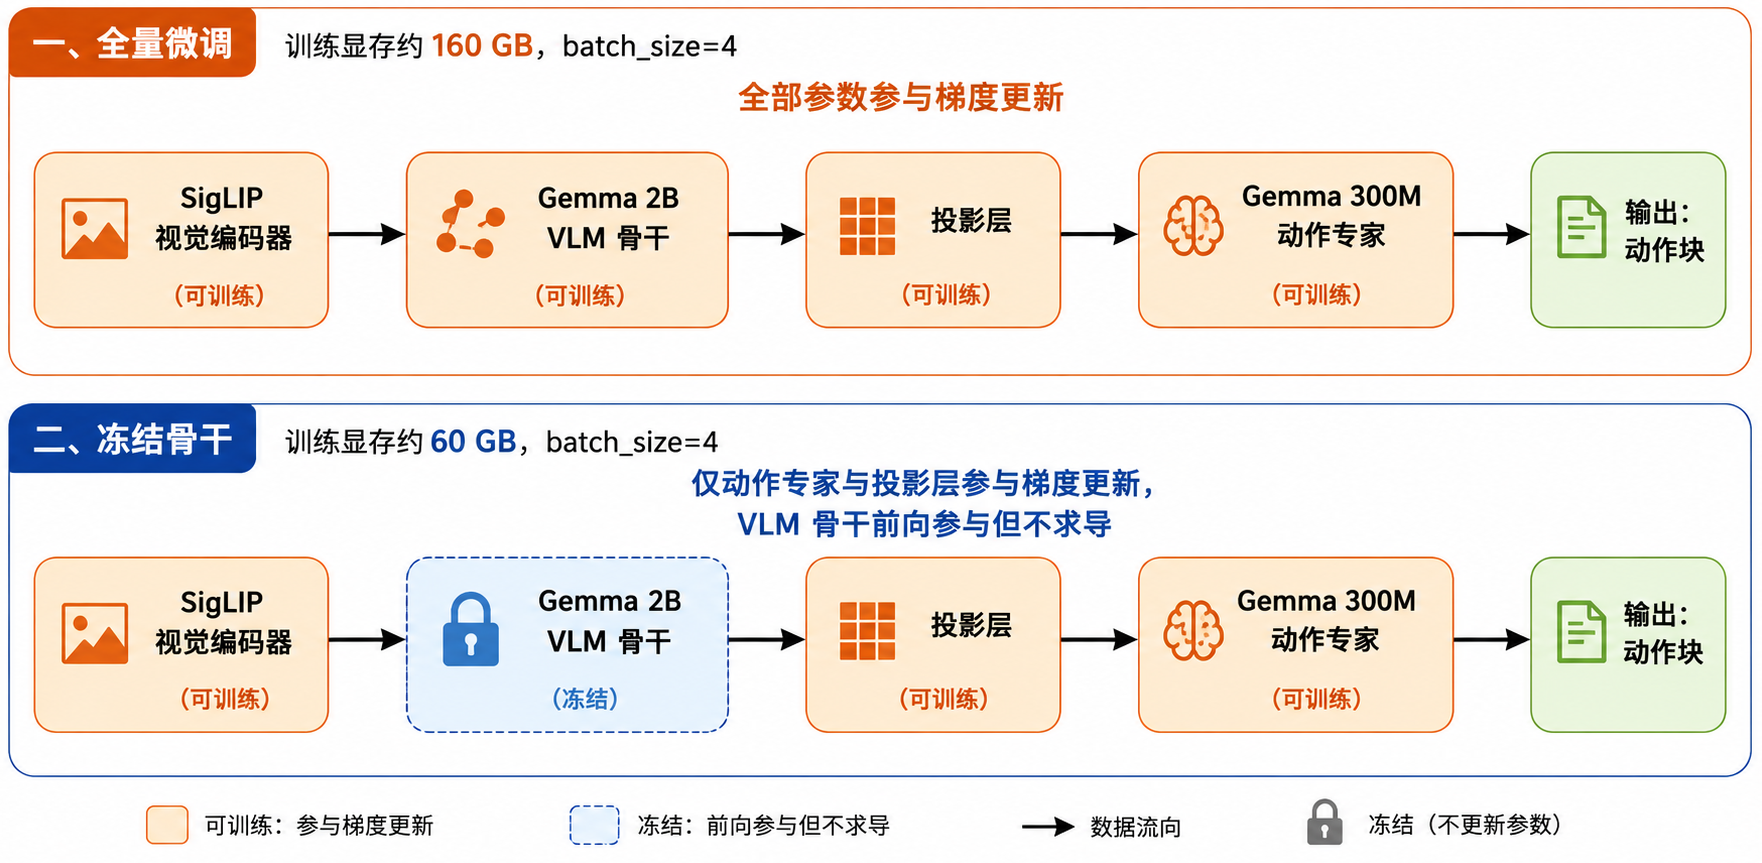
\includegraphics[width=0.88\textwidth]{images/frozen_backbone.png}
  \caption{全量微调与冻结骨干训练模式对比}
  \label{fig:frozen-backbone}
\end{figure}

在补充实验中，冻结骨干变体在 10 次实机苹果抓取测试中成功 9 次（成功率 $90\%$），较全量微调基线（$80\%$，见第三章第\ref{sec:pi05-baseline}节）提升 10 个百分点；同时训练显存占用从约 160 GB 降至约 60 GB（批次大小为 4）。成功率提升验证了小样本条件下保留预训练视觉语义先验比充分更新全部参数更有利的判断；训练显存的大幅下降显著降低了对计算设备的要求。

\section{短期记忆变体}
\label{sec:short-memory}

\subsection{问题分析：单帧视觉编码在桌面抓取中的局限}

当前 $\pi_{0.5}$ 的视觉前缀采用"按相机逐帧编码、直接拼接"的方式：每个相机的当前帧经 SigLIP 编码为 patch tokens 后，直接与语言 token 拼接送入 Gemma 主干。这种设计没有显式建模时间维度——模型在每次推理时只能"看到"当前时刻的一帧图像，完全不具备对过去数秒视觉观测的记忆能力。

对于桌面苹果抓取任务，缺乏短期视觉记忆带来的问题尤为突出：夹爪接近目标时若短暂遮挡苹果、闭合夹爪瞬间苹果发生滚动或滑移、抬升初期夹爪从边缘脱落——这些情况下，模型若能记住"片刻前苹果的确切位置"或"夹爪刚接触苹果时的相对位姿"，便更有能力生成修正动作。然而，如果沿用当前设计把过去 $K$ 帧逐帧过一次 SigLIP 再全部拼给 Gemma，每个相机的 token 数将乘以 $K$，LLM 前缀长度、prefix attention 与 KV cache 体积线性增长，推理延迟和显存占用会快速失控。

这正是 MEM 论文 C 部分要解决的核心问题：如何在视觉编码阶段就对历史帧进行压缩融合，而非把所有历史 token 都扔给 VLM 主干。

\subsection{MEM式短期记忆视频编码器的核心原理}

MEM 论文\cite{mem2025multiscale}提出的短期记忆模块，并非简单增加历史帧数量，而是在视觉编码器（SigLIP/ViT）内部引入时间维度建模，通过空间-时间可分离注意力（Space-Time Separable Attention）在保留当前帧空间细节的同时，以极低的 token 开销压缩历史视觉信息。其核心机制包括以下三个层面。

(1) 时间位置编码与预训练权重对齐。

对第 $l$ 层、空间 patch $p$、时间步 $t$ 的输入 token $z^{l-1}_{p,t}$，加入仅依赖时间步的正弦位置编码：
\begin{equation}
  \hat{z}^{l-1}_{p,t} = z^{l-1}_{p,t} + e(t),
  \label{eq:temporal-pos-enc}
\end{equation}
其中 $e(t)$ 为 sinusoidal embedding，且强制满足边界条件 $e(0)=0$。这一条件使得"当前帧"（$t=0$）的表示与原单帧 SigLIP 编码完全一致，从而最大限度地继承预训练 ViT 的视觉能力。

(2) 空间-时间可分离注意力。

论文将视频注意力分解为两步可分离操作——先做时间方向注意力，再做空间方向注意力：
\begin{equation}
  \alpha^{l,a}_{p,t}\big(S=\{1,\dots,N\},\,T=\emptyset\big)\;
  \Big[\alpha^{l,a}_{p,t}\big(S=\emptyset,\,T=\{1,\dots,T\}\big)[\hat{z}]\Big],
  \label{eq:space-time-separable}
\end{equation}
其中 $S$ 和 $T$ 分别表示空间和时间索引集合。工程上，时间注意力（因果）对同一 patch 位置 $p$ 沿时间轴做因果 attention（$t' \leq t$），确保训练时不泄漏未来帧信息；空间注意力（双向）对同一时间步 $t$ 在所有 $N$ 个 patch 上做标准双向 attention。

Q/K/V 投影矩阵直接复用原始 SigLIP 每层每头的参数，视频化主要发生在注意力连接方式的改变上，而非彻底重训新主干。实现上通过张量形状变换即可复用现有多头注意力：时间注意力将 token 序列重塑为 $(B\times N,\,K,\,D)$ 后在 $K$ 个时间步上做因果注意力，空间注意力将 token 序列重塑为 $(B\times K,\,N,\,D)$ 后在 $N$ 个图块上做双向注意力。

(3) 历史 token 压缩：当前帧全量 + 历史帧池化摘要。

论文正文图 4 与附录 C 还强调了 token 压缩策略——在较高层逐步丢弃过去时间步的 observation tokens，只保留更少、更抽象的历史 token 传给 VLM 主干。本文采用"当前帧保留全部 $N$ 个 patch tokens + 每个历史帧仅保留 $M$ 个池化摘要 tokens（$M \ll N$）"的策略，通过可学习的 pooling 将过去帧压缩为少量 memory tokens。

\subsection{本文实现与关键参数}

本文在 OpenPI/$\pi_{0.5}$ 框架中新增了视频编码模块，在 SigLIP 的图块嵌入与空间注意力层权重基础上，增加时间位置编码与空间-时间可分离注意力，最终输出压缩后的视觉记忆 tokens 供前缀构造使用。该模块的关键配置参数如表~\ref{tab:memory-config} 所示，其工作原理如图~\ref{fig:short-term-memory} 所示。

\begin{table}[htbp]
  \centering
  \small
  \caption{短期记忆模块关键配置}
  \label{tab:memory-config}
  \begin{tabular}{>{\raggedright\arraybackslash}p{5.2cm}>{\raggedright\arraybackslash}p{2.4cm}>{\raggedright\arraybackslash}p{5.6cm}}
    \toprule
    参数 & 取值 & 含义 \\
    \midrule
    记忆窗口帧数 & 4 & 模型可访问最近约 0.4--0.5 秒内的视觉历史 \\
    历史帧采样间隔 & 1（控制步） & 连续帧无跳帧，保证时序连续性 \\
    每历史帧保留的池化摘要 token 数 & 8 & 相较单帧约 256 个 patch token 实现约 32 倍压缩 \\
    当前帧保留策略 & 全部 patch tokens & 保证抓取接触阶段的细粒度空间精度 \\
    施加时间注意力的层数 & 4 & 在 SigLIP 的若干中间层施加因果时间注意力 \\
    启用短期记忆的相机 & 腕部相机 & 遮挡恢复和抓取修正主要依赖腕部手眼视角 \\
    \bottomrule
  \end{tabular}
\end{table}

\begin{figure}[htbp]
  \centering
  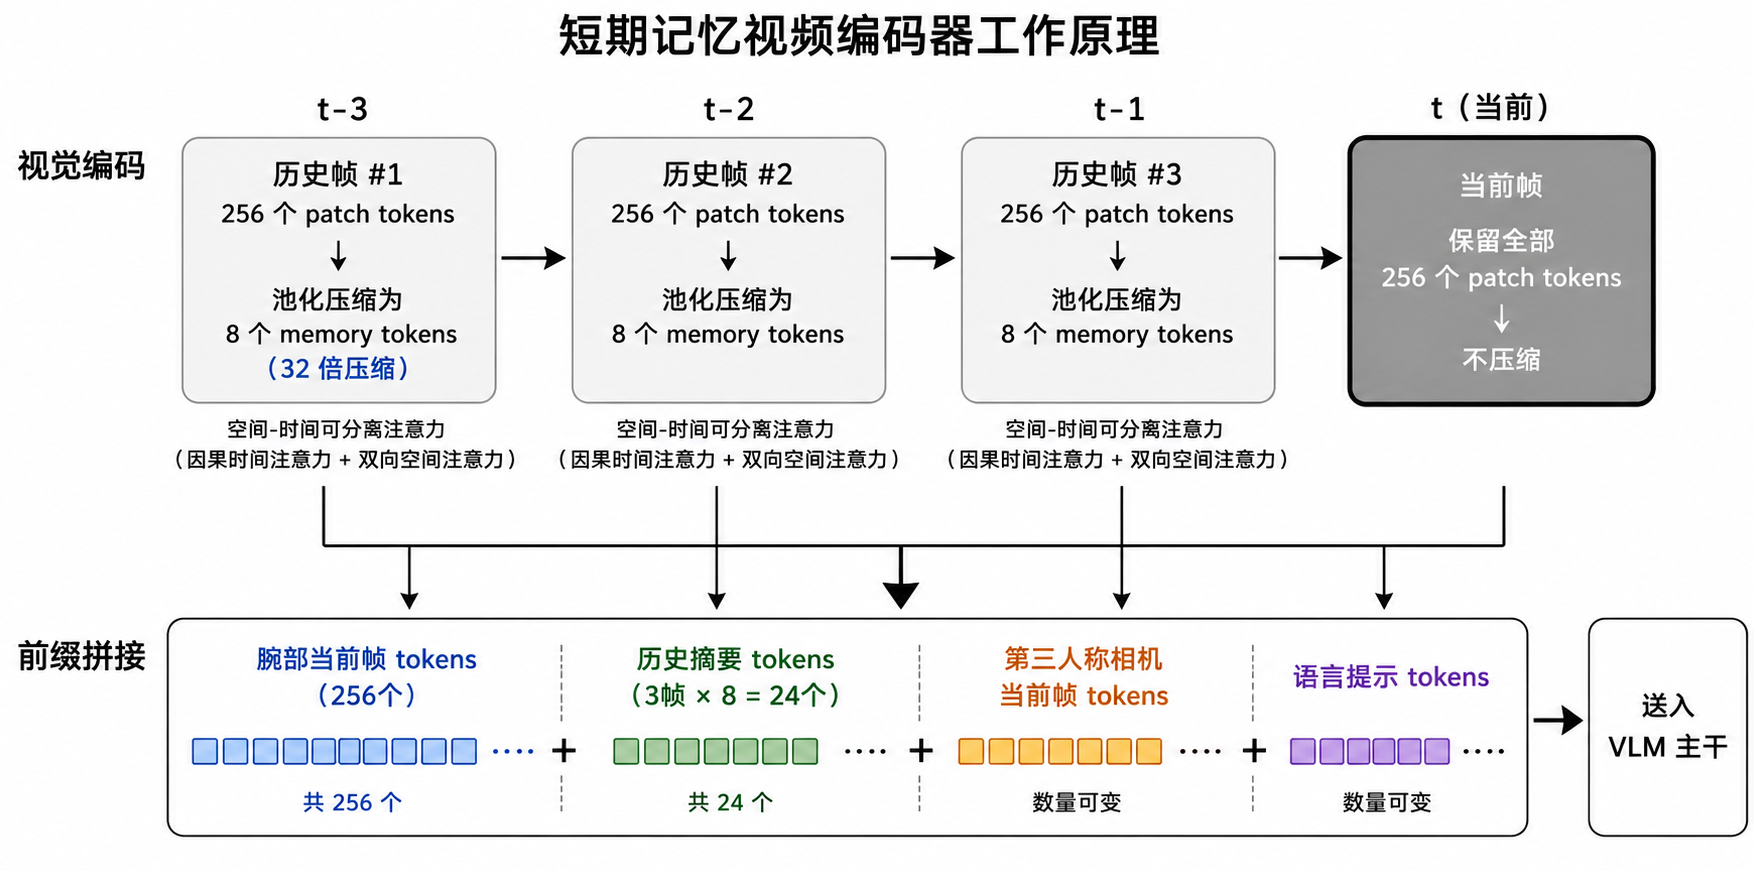
\includegraphics[width=0.88\textwidth]{images/short_term_memory.png}
  \caption{短期记忆视频编码器工作原理}
  \label{fig:short-term-memory}
\end{figure}

其中，4 帧记忆窗口与帧间隔为 1 意味着模型能访问最近约 0.4--0.5 秒内的视觉历史；每历史帧仅保留 8 个池化 token，相较单帧约 256 个 patch token 实现了约 32 倍压缩；当前帧保留全部 patch token 以保证抓取接触阶段的细粒度空间精度。初始版本仅对腕部相机启用短期记忆，因为遮挡恢复和抓取修正主要依赖腕部手眼视角的局部几何信息。

前缀拼接后结构为：
\begin{equation}
  \underbrace{[\text{cam}_{\text{wrist}}\;\text{当前帧 tokens} + \text{历史摘要 tokens}]}_{\text{视频记忆编码器输出}} + [\text{cam}_{\text{base}}\;\text{当前帧 tokens}] + [\text{prompt tokens}],
  \label{eq:prefix-with-memory}
\end{equation}
其中视频记忆编码器输出的历史摘要 tokens 远少于将原始 $K$ 帧全部展开的 token 数，从而在不显著增加 LLM 前缀长度的前提下为模型提供短期视觉记忆。

\subsection{行为效应与实验验证}

从行为层面看，短期记忆视频编码器带来了三个方面的提升。一是增强遮挡鲁棒性：当夹爪短暂遮挡目标苹果时，模型可通过历史帧中未被遮挡的苹果位置信息继续引导末端接近，而非在失去目标视觉后立即进入随机搜索。二是改善接触阶段修正能力：夹取瞬间若苹果发生滑移或滚动，历史帧中记录的位置变化使模型能够感知位移方向并生成相应的末端调整动作。三是自然形成失败恢复能力：一旦初次夹取失败（如苹果从指尖滑落），近期的视觉记忆使模型仍能定位苹果的当前位置，自主生成"重新搜索--对准--夹取"的恢复动作序列，而非在失败轨迹上继续执行无效动作。

尤为重要的是，短期记忆变体并未引入显式的失败检测模块、额外的重试逻辑或人工设计的恢复轨迹。这种自发失败恢复能力的涌现，完全来自视觉编码器对近期视觉历史的压缩融合——模型在条件输入层面就获得了对"刚才发生了什么"的感知。在补充实验中，短期记忆变体在 10 次实机测试中成功 10 次（$100\%$），并在多次初次夹取失败后自主完成了再搜索与再夹取。

从更宏观的视角看，短期记忆变体的有效性揭示了一个对桌面 VLA 部署具有普遍意义的洞察：对于接触富集、短周期闭环主导的任务，在视觉编码阶段而非 LLM 前缀阶段压缩历史信息，能够以更低的计算代价获得更强的在线修正能力。这一发现与第 \ref{sec:pi05-deploy} 节中分段闭环执行策略的成功率提升（从约 $5\%$ 至接近 $100\%$）形成互补——前者从模型结构层面增强了对近期视觉信息的利用效率，后者从部署策略层面确保了推理结果能够及时响应最新观测。

\section{模型变体综合对比与启示}
\label{sec:variant-comparison}

表~\ref{tab:variant-analysis} 对本文三类模型变体的实验效果做了归纳对比。

\begin{table}[htbp]
  \centering
  \small
  \caption{模型变体效果对比}
  \label{tab:variant-analysis}
  \begin{tabular}{>{\raggedright\arraybackslash}p{3.0cm}>{\raggedright\arraybackslash}p{1.9cm}>{\raggedright\arraybackslash}p{3.5cm}>{\raggedright\arraybackslash}p{4.4cm}}
    \toprule
    模型变体 & 结论性质 & 主要特点 & 预期/观察效果 \\
    \midrule
    基础版 $\pi_{0.5}$ 微调模型 & 已观察 & 能力完整，适合作为主基线 & 10 次抓取成功 8 次，成功率约 $80\%$；训练显存约 160 GB，推理显存约 $12\,\mathrm{GB}$ \\
    冻结视觉语言主干，仅调动作专家 & 已观察 & 训练代价低，保留原始语义先验 & 10 次抓取成功 9 次，成功率约 $90\%$；训练显存约 60 GB，推理显存约 $12\,\mathrm{GB}$ \\
    冻结视觉编码器，微调其余模块 & 预估 & 适合固定视角、固定对象类别场景 & 可能在小数据条件下取得较好的精度/成本折中 \\
    短期记忆 $\pi_{0.5}$ & 已观察 + 机理分析 & 视觉编码器中引入空间-时间可分离注意力与历史token压缩，提供短期视觉记忆 & 10 次抓取成功 10 次，成功率 $100\%$；训练显存约 160 GB，推理显存约 $12\,\mathrm{GB}$，并表现出较强失败恢复能力 \\
    \bottomrule
  \end{tabular}
\end{table}

图~\ref{fig:variant-success-memory} 以柱状图直观对比三类变体的成功率与训练显存占用（批次大小为 4）：冻结主干变体在保持 $90\%$ 成功率的同时将训练显存从约 160 GB 降至约 60 GB，三类变体推理显存一致（均约 12 GB）。

\begin{figure}[htbp]
  \centering
  \small
  \begin{tabular}{cc}
    \begin{tikzpicture}[x=1cm,y=0.03cm]
      \draw[->] (0,0) -- (0,110) node[above] {成功率/\%};
      \draw[->] (0,0) -- (4.4,0);
      \foreach \y in {0,20,40,60,80,100} {
        \draw (-0.06,\y) -- (0,\y) node[left] {\y};
      }
      \fill[black!55] (0.45,0) rectangle (0.95,80);
      \fill[black!35] (1.85,0) rectangle (2.35,90);
      \fill[black!75] (3.25,0) rectangle (3.75,100);
      \node[above] at (0.70,80) {$80$};
      \node[above] at (2.10,90) {$90$};
      \node[above] at (3.50,100) {$100$};
      \node[below,align=center] at (0.70,-7) {全量\\微调};
      \node[below,align=center] at (2.10,-7) {冻结\\主干};
      \node[below,align=center] at (3.50,-7) {短期\\[3pt]记忆};
    \end{tikzpicture}
    &
    \begin{tikzpicture}[x=1cm,y=0.02cm]
      \draw[->] (0,0) -- (0,170) node[above] {训练显存/GB};
      \draw[->] (0,0) -- (4.4,0);
      \foreach \y in {0,40,80,120,160} {
        \draw (-0.06,\y) -- (0,\y) node[left] {\y};
      }
      \fill[black!55] (0.45,0) rectangle (0.95,160);
      \fill[black!35] (1.85,0) rectangle (2.35,60);
      \fill[black!75] (3.25,0) rectangle (3.75,160);
      \node[above] at (0.70,160) {$160$};
      \node[above] at (2.10,60) {$60$};
      \node[above] at (3.50,160) {$160$};
      \node[below,align=center] at (0.70,-1.2) {全量\\微调};
      \node[below,align=center] at (2.10,-1.2) {冻结\\主干};
      \node[below,align=center] at (3.50,-1.2) {短期\\[3pt]记忆};
    \end{tikzpicture}
  \end{tabular}
  \caption{三类模型变体成功率与显存对比}
  \label{fig:variant-success-memory}
\end{figure}

从上述对比中可以得到两点启示。

第一，桌面抓取任务更依赖短周期闭环修正，而不是长时间开环规划。
因此，无论是部署时采用分段执行，还是训练时引入更适合失败恢复的记忆结构，本质上都是在增强"看见当前状态后迅速修正动作"的能力。

第二，小样本专用任务中的最优模型，不一定是参数更新最多的模型。
对于 30 条示教数据这样的小规模任务，冻结部分主干、仅微调动作专家或少量适配参数，
已经在补充实验中表现出更低训练显存占用和较高抓取成功率，说明其很可能在训练资源与最终性能之间取得更好的平衡。未来如果继续扩展数据量、增加苹果种类、
改变桌面背景或加入更多失败恢复示教，再对这些变体做定量对比，将有助于形成更完整的桌面 VLA 训练经验。
